\documentclass[12pt,a4paper]{article}
\usepackage[czech]{babel}
\usepackage[utf8]{inputenc}
\usepackage[T1]{fontenc}
\usepackage{graphicx}
\usepackage{enumitem}
\usepackage{titling}
\usepackage{graphicx}
\textwidth 16cm \textheight 24.6cm
\topmargin -1.3cm
\oddsidemargin 0cm
\begin{document}
\thispagestyle{empty}

\setlength{\parindent}{0cm}
\setlength{\parskip}{1mm plus2pt minus1pt}

\setlength{\droptitle}{-5em}

\title{
\Large Ovládání kolejiště pomocí hJOP\\
\LARGE Podklady pro zkoušku oprávnění řízení\\
\small v2.0-alpha}
\author{Jan Horáček (jan.horacek@kmz-brno.cz)}
\date{\today}
\maketitle

Tento dokument obsahuje podklady pro učení a testování způsobilosti řízení
hJOP. Jeho cílem je nastavit jednotnou míru znalostí obsluhy kolejiště a~tím
předejít zbytečným chybám, zdržování provozu, újmám na majetku a~přispět
k~obecně lepší součinnosti mezi obsluhou kolejiště.

Následující text obsahuje několik úrovní zaškolení – od základní až po tu
nejpokročilejší. Každá úroveň obsahuje teoretické otázky a~praktickou část, ve
které probíhá řešení zadaných úkolů přímo na kolejišti. Každý, kdo chce získat
příslušné oprávnění, musí odpovědět na všechny otázky a~být schopen vyřešit
všechny praktické problémy. Otázky v~jednotlivých sekcích jsou seřazeny od
nejdůležitějších k~méně důležitým.

\section{Doporučená metodika zaškolování}

\begin{enumerate}[leftmargin=*]
\item Nováčka zařadit k~někomu (patronovi) na úrovni, kterou požaduje, ten ho
naučí základy obsluhy.
\item Nováčkovi dát k~dispozici tento dokument, on si přečte dotazy, případné
nejasnosti vyřeší se zaškoleným patronem.
\item Oprávnění získává nováček výhradně u~školitele – u~kohokoliv s~oprávněním
A. Školitel vybere otázky z~tohoto dokumentu a~nechá nováčka odpovědět. Školitel
provede s~no\-váč\-kem praktickou část zkoušky.
\item Školitel přidává login nováčka do hJOPserveru, nováček je oprávněn řídit.
\end{enumerate}

\newpage

\section{S0 – strojvedoucí hJOPdriver}

Opravňuje k~řízení vlaků přes mobilní aplikaci hJOPdriver.

\subsection{Praktická část}

\begin{enumerate}[leftmargin=*]
\item Proveďte převzetí vlaku na ruční řízení.
\item Proveďte uvolnění vlaku z~aplikace.
\item Demonstrujte řízení lokomotiv v~multitrakci.
\item Vysvětlete obsah sešitového jízdního řádu.
\item Demonstrujte komunikaci s~výpravčím.
\item Demonstrujte poznání trati, ukažte polohy jednotlivých návěstidel.
\end{enumerate}

\subsection{Teoretická část}
\begin{enumerate}[leftmargin=*]
\item Jaký je rozdíl mezi ručním řízením a totálním ručním řízením?
\item Kdy má v~řízení jízdy přednost ovladač a kdy počítač?
\item Pouští počítač automaticky funkce houkání apod., když je HV na ovladači?
\item Jaká specifika platí pro řízení jízdy vlaku s~více lokomotivami v~multitrakci?
\item Popište jak poznáte, kam až smíte s vlakem jet.
\item Co se stane při ztrátě wifi spojení?
\item Co se stane při otevření jiné aplikace?
\item Co se stane při přetočení displaye?
\end{enumerate}

\newpage

\section{S1 – dispečer základní}

Opravňuje k~řízení menších stanic.

Pro tuto úroveň zaškolení je doporučeno mít zaškolení na úrovni S0. Výjimkou
je situace, kdy dispečeři používají k řízení jízdy jiné prostředky, než mobilní
aplikaci hJOPdriver.

\subsection{Praktická část}

\subsubsection*{Přihlášení, odhlášení}
\begin{enumerate}[leftmargin=*]
\item Spusťte panel. Připojte se k~serveru, přihlaste se, odpojte se od
serveru. Přihlaste se v~režimu čtenáře, Demonstrujte přihlášení více panelů.
\item Proveďte přihlášení k~jednomu panelu a ke všem spuštěným panelům.
\item Zobrazte a skryjte popisky bloků.
\end{enumerate}

\subsubsection*{Základní obsluha vlaků}
\begin{enumerate}[leftmargin=*]
\item Obslužte několik vlaků.
\item Proveďte křižování osobních vlaků.
\end{enumerate}

\subsubsection*{Dopravní kancelář}
\begin{enumerate}[leftmargin=*]
\item Demonstrujte komunikaci se sousedními dispečery (telefon, poslání zprávy).
\item Demonstrujte přepnutí řízení na místní a dálkový provoz.
\end{enumerate}

\subsubsection*{Soupravy}
\begin{enumerate}[leftmargin=*]
\item Proveďte vytvoření soupravy.
\item Proveďte smazání soupravy.
\item Zobrazte seznam souprav v~obvodech všech vámi řízených stanic, vysvětlete
význam tohoto seznamu.
\item Upravte výchozí a cílovou stanici soupravy v koncové stanici.
\end{enumerate}

\subsubsection*{Bloky}
\begin{enumerate}[leftmargin=*]
\item Proveďte ruční přestavení výhybky.
\item Proveďte nouzové ruční přestavení výhybky.
\item Vyřešte uváznutý vagón v~trati.
\item Proveďte nouzové uvolnění závěrů úseků. Vysvětlete, kdy se takové uvolnění
provádí.
\item Demonstrujte obsluhu rozpojovačů.
\item Zaveďte štítek na úseku.
\end{enumerate}

\subsubsection*{Jízdní cesty}
\begin{enumerate}[leftmargin=*]
\item Proveďte zrušení JC. Ukažte co nejvíce postupů.
\item Demonstrujte posun ve stanici.
\item Proveďte obsluhu vlaku v~ručním režimu řízení, včetně stavění jízdních
cest.
\end{enumerate}

\subsubsection*{Ruční řízení}
\begin{enumerate}[leftmargin=*]
\item Předveďte ruční řízení vlaku přes aplikaci Jerry.
\item Předveďte komunikaci se strojvedoucím.
\item Demonstrujte násilné převzetí soupravy od strojvedoucího.
\end{enumerate}

\subsubsection*{Krizové scénáře}
\begin{enumerate}[leftmargin=*]
\item Proveďte nouzové zastavení provozu na celém kolejišti.
\item Proveďte nouzové zastavení jedné lokomotivy.
\item Vyřešte situaci, kdy vlak přejel do následujícího kolejového obvodu.
\item Vyřešte situaci, kdy vlak rozřezal výhybku a způsobil zkrat.
\end{enumerate}

\subsubsection*{Poznání}
\begin{enumerate}[leftmargin=*]
\item Demonstrujte poznání trati, ukažte polohy jednotlivých návěstidel, typy
traťových zabezpečovacích zařízení.
\end{enumerate}


\subsection{Teoretická část}

\subsubsection*{Přihlašování, odhlašování}
\begin{enumerate}[leftmargin=*]
\item Vysvětlete, jak funguje mechanismus přihlašování k~více panelům zároveň.
Kdy tento mechanismus použít a~kdy naopak ne?
\item Jak poznáte, že je panel připojen k~serveru?
\item Vysvětlete význam přepnutí stanice na místní a dálkový provoz.
\item Popište postup přebírání stanice jiným dispečerem, například při změně
směn.
\item Chcete se přihlásit ke stanici pouze na dívání, jak to provedete?
\item Jak potlačíte zvukovou notifikaci zkratu na kolejišti? Je toto potlačení
trvalé?
\item Můžete z~libovolného pracoviště ovládat libovolnou stanici?
\item Jakými všemi metodami mohu komunikovat s~dispečery sousedních stanic?
\item Ke kolejišti přijde váš kamarád, který si chce zajezdit, ale nemá
zaškolení (nemá login), co mu můžete povolit a co naopak nesmíte? Jak se k~němu
máte chovat?
\end{enumerate}

\subsubsection*{Soupravy}
\begin{enumerate}[leftmargin=*]
\item Jaký je rozdíl mezi vlakem, lokomotivou a~soupravou? Může se lokomotiva
sama pohybovat na širé trati?
\item Jak poznáte typ blížícího se vlaku? Jaká rozhodnutí na základě typu
typicky děláte?
\item Vyjmenujte, jaká předčíslí souprav mají jaký význam.
\item Jaké je typické složení čísla vlaku? Jak poznat z~čísla vlaku adresu
lokomotivy?
\item Vysvětlete rozdíl mezi směrem vlaku a směrem stanoviště A.
\item Jak poznat, že má vlak správně zadáno stanoviště A?
\item Kdy je a kdy není třeba upravovat výchozí a cílovou stanici?
\item Kolik lokomotiv může mít souprava?
\item Je nutné měnit orientaci stanoviště A~při otáčení vlaku v~koncové
stanici?
\item Je nutné zadávat vlaku jeho délku a~typ? Proč?
\item Na které místo ve vlaku je možné přivěsit čistící vůz?
\end{enumerate}

\subsubsection*{Bloky}
\begin{enumerate}[leftmargin=*]
\item Jak poznáte zkrat na kolejišti? Co s~ním dělat?
\item Vysvětlete význam následujících symbolů na reliéfu. \\
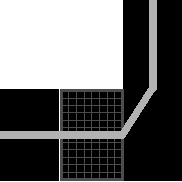
\includegraphics[width=0.1\textwidth]{symboly/kol1.png}
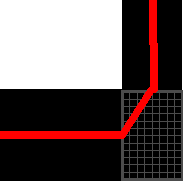
\includegraphics[width=0.1\textwidth]{symboly/kol2.png}
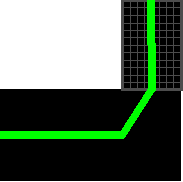
\includegraphics[width=0.1\textwidth]{symboly/kol3.png}
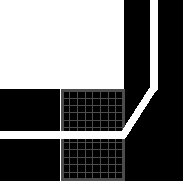
\includegraphics[width=0.1\textwidth]{symboly/kol4.png}

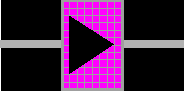
\includegraphics[width=0.1\textwidth]{symboly/hlnav16.png}
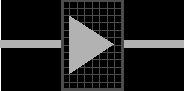
\includegraphics[width=0.1\textwidth]{symboly/hlnav1.png}
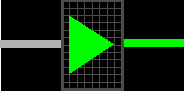
\includegraphics[width=0.1\textwidth]{symboly/hlnav2.png}
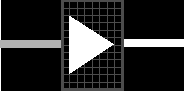
\includegraphics[width=0.1\textwidth]{symboly/hlnav3.png}
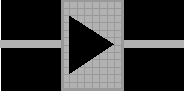
\includegraphics[width=0.1\textwidth]{symboly/hlnav5.png}
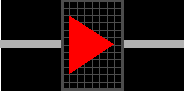
\includegraphics[width=0.1\textwidth]{symboly/hlnav6.png}
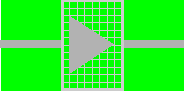
\includegraphics[width=0.1\textwidth]{symboly/hlnav8.png}

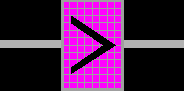
\includegraphics[width=0.1\textwidth]{symboly/senav6.png}
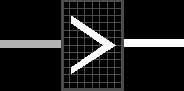
\includegraphics[width=0.1\textwidth]{symboly/senav2.png}
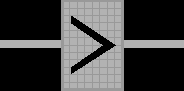
\includegraphics[width=0.1\textwidth]{symboly/senav3.png}
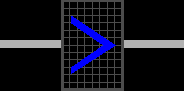
\includegraphics[width=0.1\textwidth]{symboly/senav4.png}

\includegraphics[width=0.1\textwidth]{symboly/senav8.png}

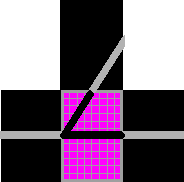
\includegraphics[width=0.1\textwidth]{symboly/vyh4.png}
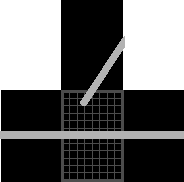
\includegraphics[width=0.1\textwidth]{symboly/vyh1.png}
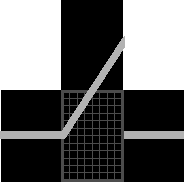
\includegraphics[width=0.1\textwidth]{symboly/vyh2.png}
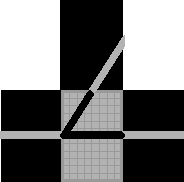
\includegraphics[width=0.1\textwidth]{symboly/vyh3.png}
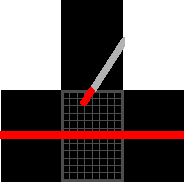
\includegraphics[width=0.1\textwidth]{symboly/vyh5.png}

\includegraphics[width=0.1\textwidth]{symboly/vyh6.png}
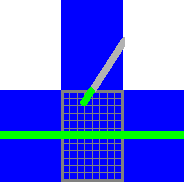
\includegraphics[width=0.1\textwidth]{symboly/vyh28.png}
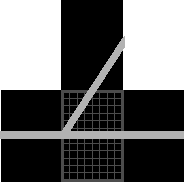
\includegraphics[width=0.1\textwidth]{symboly/vyh37.png}
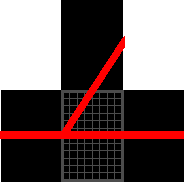
\includegraphics[width=0.1\textwidth]{symboly/vyh38.png}
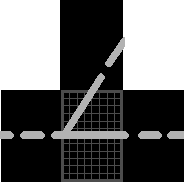
\includegraphics[width=0.1\textwidth]{symboly/vyh39.png}

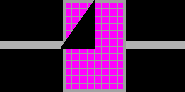
\includegraphics[width=0.1\textwidth]{symboly/vyk19.png}
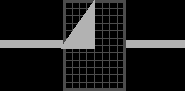
\includegraphics[width=0.1\textwidth]{symboly/vyk1.png}
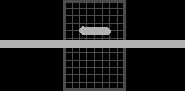
\includegraphics[width=0.1\textwidth]{symboly/vyk2.png}
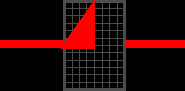
\includegraphics[width=0.1\textwidth]{symboly/vyk3.png}
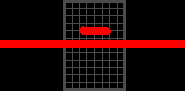
\includegraphics[width=0.1\textwidth]{symboly/vyk4.png}
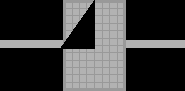
\includegraphics[width=0.1\textwidth]{symboly/vyk5.png}
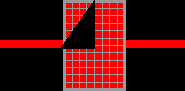
\includegraphics[width=0.1\textwidth]{symboly/vyk6.png}

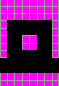
\includegraphics[width=0.05\textwidth]{symboly/ez6.png}

\includegraphics[width=0.05\textwidth]{symboly/ez1.png}

\includegraphics[width=0.05\textwidth]{symboly/ez2.png}

\includegraphics[width=0.05\textwidth]{symboly/ez3.png}
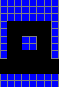
\includegraphics[width=0.05\textwidth]{symboly/ez5.png}

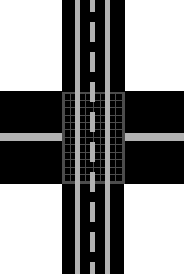
\includegraphics[width=0.1\textwidth]{symboly/prej1.png}
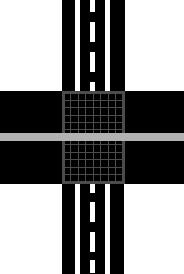
\includegraphics[width=0.1\textwidth]{symboly/prej2.png}
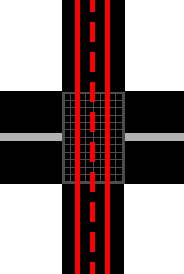
\includegraphics[width=0.1\textwidth]{symboly/prej3.png}

\item Kdy je a kdy není nutné žádat o~traťový souhlas?
\item Co je to závěr a k~čemu slouží?
\item Sousední stanice mě žádá o~traťový souhlas, vy ho však chcete přijmout až
za minutu, jak nejlépe sdělit sousední stanici, že má počkat?
\item Jak poznáte dopravní a manipulační kolej?
\item Jak poznáte směr trati na reliéfu?
\item Úvazka je červená, co to znamená?
\end{enumerate}

\subsubsection*{Jízdní cesty}
\begin{enumerate}[leftmargin=*]
\item Má mít vlak v~ručním řízení postavenou jízdní cestu pro jízdu na
kolejišti?
\item Jak mohu zrušit jízdní cestu? Popište co nejvíce metod.
\item Popište vztah mezi pojmy \textit{jízdní cesta}, \textit{vlaková cesta} a
\textit{posunová cesta}.
\end{enumerate}

\subsubsection*{Ruční řízení}
\begin{enumerate}[leftmargin=*]
\item Vyjmenujte všechny možnosti, jak řídit lokomotivu ručně.
\item Co znamená, když je v~regulátoru zaškrtnuto \textit{totální ruční řízení}
a k~čemu mě to opravňuje?
\end{enumerate}

\subsubsection*{Krizové scénáře}
\begin{enumerate}[leftmargin=*]
\item Jako posunovač máte volnou chvíli, ohlédnete se do sousední stanice a
vidíte, že dva vlaky jedou proti sobě a nezpomalují, přibližně za 5 s~do sebe
narazí. Co uděláte?
\item Kdy použít nouzové zastavení celého kolejiště a kdy vybrané soupravy?
\end{enumerate}

\subsubsection*{Odpovědnost}
\begin{enumerate}[leftmargin=*]
\item Popište, za co jako dispečer odpovídáte.
\item Co dělat, když na kolejišti něco rozbijete?
\end{enumerate}

\subsubsection*{Vlakotvorba}
\begin{enumerate}[leftmargin=*]
\item Popište, podle čeho se rozhodujete jaký vlak kdy a kam poslat.
\item Kde se dozvíte, co stanice vyváží a dováží?
\item Které úkony je nutné vykonat k~řádnému zpracování manipulačního vlaku,
který vám právě přijel do stanice? Zpracování manipulačního vlaku končí
v~momentě jeho odjezdu ze stanice.
\item Potřebujete lokomotivní zálohu z~výtopny/depa, jak ji získáte?
\item Co to znamená, že se na kolejišti \textit{jezdí nákladní doprava} a~jak
nákladní doprava funguje?
\item Kam píšete nákladní vozy ve vlaku?
\end{enumerate}

\subsubsection*{Další}
\begin{enumerate}[leftmargin=*]
\item Co je to riziková funkce?
\item Které všechny úkony je nutné vykonat při potvrzování rizikové funkce?
Uveďte na příkladu nouzového stavění výhybky.
\end{enumerate}


\newpage
\section{S1u – dispečer řízení jízdy přes uLI}

Musí být součástí zaškolení úrovně S1 pro kolejiště, kde se používají
uLI-daemon.

\subsection{Praktická část}

\begin{enumerate}[leftmargin=*]
\item Proveďte převzetí, řízení a uvolnění soupravy na Roco Multimaus.
\end{enumerate}

\subsection{Teoretická část}

\begin{enumerate}[leftmargin=*]
\item Co je to \textit{uLI-daemon} a~jakou má funkci?
\item Co je to \textit{uLI-master} a~jakou má funkci?
\item Ikonka mašinky na Rocomaus bliká, co to znamená?
\item Ikonka mašinky na Rocomaus trvale svítí, mašinka přesto nereaguje, co je
špatně?
\end{enumerate}


\newpage
\section{S2 – pokročilý dispečer}

Opravňuje k~řízení větších stanic. Obsahuje otázky na veškerou funkcionalitu,
kterou umí hJOP nabídnout.

\subsection{Praktická část}

\begin{enumerate}[leftmargin=*]
\item Demonstrujte zapnutí a~vypnutí kolejiště a~serveru.
\item Rozsviťte přivolávací návěst na návěstidle bez postavení nouzové cesty.
\item Proveďte příjem vlaku na obsazenou kolej včetně zrušení nouzové cesty.
\item Ručně uzavřete přejezd.
\item Proveďte nouzové otevření přejezdu.
\item Vytvořte a zrušte soupravu s~více lokomotivami.
\item Přidejte na kolej více souprav.
\item Přesuňte soupravu na jinou kolej.
\item Prohoďte soupravy na jedné koleji.
\item Proveďte vytvoření nové lokomotivy.
\item Proveďte úpravu dat lokomotivy.
\item Zjistěte, kde se nachází lokomotiva s~danou adresou.
\item Nastavte modelový čas, zapněte jej a vypněte jej.
\item Předveďte práci se zásobníkem povelů: přidání povelu, pozastavení
zásobníku, smazání povelu, přesun povelů.
\item Proveďte maximálně možně zabezpečený nouzový vjezd vlaku na manipulační
kolej.
\item Demonstrujte multitrakci v~ručním ovladači.
\item Zaveďte předvídaný odjezd vlaku.
\item Zaveďte na návěstidle režim AB, zrušte režim AB.
\item Postavte JC s variantními body.
\item Postavte složenou JC s~variantními body.
\end{enumerate}

\newpage
\subsection{Teoretická část}

\begin{enumerate}[leftmargin=*]
\item Vysvětlete význam náslědujících symbolů. \\
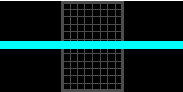
\includegraphics[width=0.1\textwidth]{symboly/kol5.png}
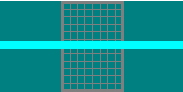
\includegraphics[width=0.1\textwidth]{symboly/kol7.png}
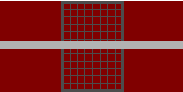
\includegraphics[width=0.1\textwidth]{symboly/kol8.png}

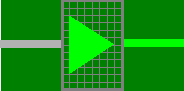
\includegraphics[width=0.1\textwidth]{symboly/hlnav9.png}

\includegraphics[width=0.1\textwidth]{symboly/hlnav15.png}
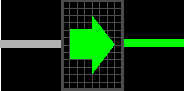
\includegraphics[width=0.1\textwidth]{symboly/hlnav17.png}
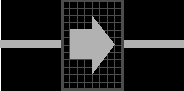
\includegraphics[width=0.1\textwidth]{symboly/hlnav18.png}
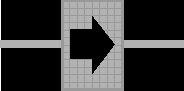
\includegraphics[width=0.1\textwidth]{symboly/hlnav19.png}

\includegraphics[width=0.1\textwidth]{symboly/senav14.png}

\includegraphics[width=0.1\textwidth]{symboly/vyh7.png}
\includegraphics[width=0.1\textwidth]{symboly/vyh8.png}
\includegraphics[width=0.1\textwidth]{symboly/vyh14.png}
\includegraphics[width=0.1\textwidth]{symboly/vyh21.png}
\includegraphics[width=0.1\textwidth]{symboly/vyh22.png}
\includegraphics[width=0.1\textwidth]{symboly/vyh23.png}
\includegraphics[width=0.1\textwidth]{symboly/vyh24.png}
\includegraphics[width=0.1\textwidth]{symboly/vyh25.png}
\includegraphics[width=0.1\textwidth]{symboly/vyh26.png}
\includegraphics[width=0.1\textwidth]{symboly/vyh27.png}

\includegraphics[width=0.1\textwidth]{symboly/vyk9.png}
\includegraphics[width=0.1\textwidth]{symboly/vyk10.png}
\includegraphics[width=0.1\textwidth]{symboly/vyk11.png}
\includegraphics[width=0.1\textwidth]{symboly/vyk17.png}

\includegraphics[width=0.05\textwidth]{symboly/ez4.png}

\item Nouzové závěry kterých bloků se automaticky neruší při volbě \textit{RNZ
– rušení nouzových závěrů} a je třeba je zrušit ručně?
\item Jaké všechny povely lze vkládat do zásobníku povelů?
\item Zásobník povelů je přepnutý do volby \textit{PV}, je zásobník aktivní?
\item Mohu vypnout napájecí zdroj stanice za plného provozu? Co po vypnutí
napájení udělá ovládací panel?
\item Mohu při restartu hJOP nechat vlaky v~trati?
\item Na jaké úseky lze a na jaké nelze přesouvat vlaky?
\item Vysvětlete barvy soupravy předvídaného odjezdu vlaku.
\item Vysvětlete chování režimu AB u návěstidla.
\end{enumerate}

\end{document}
